\documentclass[]{beamer}

\usepackage[utf8]{inputenc}
\usepackage[portuges]{babel}
\usepackage[T1]{fontenc}
%\usepackage{hyperref}
\usepackage[]{csquotes}

\setbeamertemplate{footline}[page number]
\setbeamercovered{transparent}
\beamertemplatenavigationsymbolsempty

\def\BLACKBG{true}
%\ifdefined\BLACKBG
  \setbeamercolor{block body}{bg=normal text.bg!90!black}
  \setbeamercolor{block body example}{bg=normal text.bg!90!black}
  \setbeamercolor{block title alerted}{use={normal text,alerted text},fg=alerted text.fg!75!normal text.fg,bg=normal text.bg!75!white}
  \setbeamercolor{block title}{bg=black}
  \setbeamercolor{block title example}{use={normal text,example text},fg=example text.fg!75!normal text.fg,bg=normal text.bg!75!white}
  \setbeamercolor{fine separation line}{}
  \setbeamercolor{frametitle}{fg=brown}
  \setbeamercolor{item projected}{fg=white}
  \setbeamercolor{normal text}{bg=black,fg=white}
  \setbeamercolor{separation line}{}
  \setbeamercolor{structure}{bg=black,fg=white}
  \setbeamercolor{title}{fg=white}
  \setbeamercolor{titlelike}{fg=white}
\fi

\newcommand{\invertbgcolor}{
  \ifdefined\BLACKBG
    %\setbeamercolor{normal text}{bg=white,fg=black}
  \fi
}

\newcommand{\backbgcolor}{
  \ifdefined\BLACKBG
    %\setbeamercolor{normal text}{bg=white,fg=black}
  \fi
}


\newcommand{\obs}[1]{{
  \ifdefined\DRAFT
    \textcolor{magenta}{#1}
  \fi
}}

\def\DRAFT{true}

\author{Grupo 5: \\
  Dmitry Rocha \and \\
  Giovanna Luana \and \\
  Maria Raquel \and \\
  Romulo Cassio
}

\title{Artigo: Ser professor hoje por Vera Maria}

\institute{UFPI}

\begin{document}
  \begin{frame}
    \titlepage
  \end{frame}

  \section{A autora}

  \begin{frame}{\secname}
    \begin{columns}[T]
      \begin{column}{.5\textwidth}
        \begin{block}{}
          \blockquote[{\cite[Currículo Lattes]{_curriculo_}}]{
            \begin{itemize}
              \item Mora atualmente no Rio de Janeiro
              \item Graduação em Licenciatura e Pedagogia
              \item Aperfeiçoamento em Educação e Filosofia
              \item Doutorado em Educação
            \end{itemize}
          }
        \end{block}
      \end{column}
      \begin{column}{.5\textwidth}
        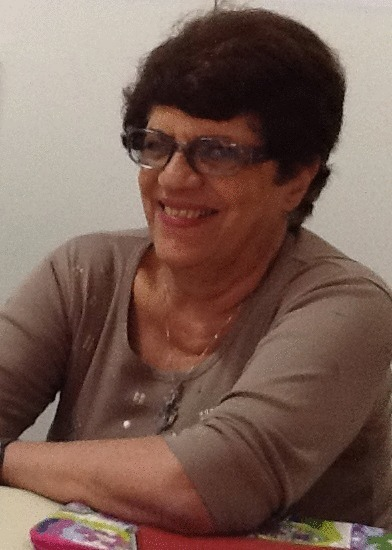
\includegraphics[scale=0.3]{foto.jpeg}
      \end{column}
    \end{columns}

    \obs{
      Todas essas informações (inclusive foto) foram tiradas do currículo
      lattes dela
    }
  \end{frame}

  \section{Resumo}

  \begin{frame}{\secname *}
    \blockquote[{\cite[
      Ser professor/a hoje: novos confrontos entre saberes, culturas e práticas
    ]{vera_maria_ferrao_candau_ser_2014}}]{
      \begin{itemize}
        \item
          Últimos anos discussão sobre a construção da identidade profissional
          dos professores e os componentes.

        \item
          Foco: analisar alguns desafios para enfrentar a perspectiva da
          exigência de ressiginificação da escola.
      \end{itemize}
    }

    \obs{
      Nota1: Falar um breve resumo do artigo, que são esses dos tópicos.
      (RESUMO, na primeira página) \\
      Nota2: Esses títulos que estão com * (canto superior esquerdo) são
      títulos do próprio artigo. Sugerir que as pessoas acompanhem na leitura
      do artigo.
    }
  \end{frame}

  \begin{frame}{Cenário}
    \begin{center}
      \Huge Hoje
    \end{center}

    \obs{
      A autora enfatiza muito que o artigo se trata do \emph{hoje} e do
      \emph{contemporâneo}, chegando até a ser prolixa. Avisar sobre isso ou
      apenas enfatizar que tudo se trata do \emph{Hoje}.
    }
  \end{frame}

  \section{Introdução}

  \begin{frame}{\secname *}
    \begin{itemize}
      \item
        A problemática atual da educação brasileira

      \item
        A pouca valorização do professor e as condições precárias de trabalho, é
        possível detectar vários problemas entre os profissionais da educação

      \item
        Novos métodos, técnicas e modernidade pode melhorar em um melhor
        desenvolvimento do aluno e professor
    \end{itemize}

    \obs{
      Acho que existe um erro no último item
    }
  \end{frame}

  \section{A Escola: Entre a 'tradição' e a reinvenção}

  \begin{frame}{\secname *}
    \begin{itemize}
      \item
        A educação renovada para melhor adequação a sociedade

      \item
        A escola vem sendo um processo institucional moderno

      \item
        A contribuição da escola e da sociedade por gerar cidadães independente
        de suas diferenças de origem

      \item
        A escola questiona seu próprio modelo de sociedade assim causando sua
        crise
    \end{itemize}
  \end{frame}

  \section{Culturas, multiculturalismos e educação}

  \begin{frame}{\secname *}
    \begin{itemize}
      \item
        Existe uma relação intrínseca entre educação e culturas

      \item
        "A escola deve ser concebida como um espaço ecológico de cruzamento de
        culturas"

      \item
        No artigo se refere a três perspectivas fundamentais:
        \begin{itemize}
          \item
            % promove uma universalização da escolarização
            Multiculturalismo assimilacionista

          \item
            Multiculturalismo diferencialista (ou monoculturalismo plural)
          \item Multiculturalismo interativo
        \end{itemize}
    \end{itemize}

    \obs{
      Se eu for escolhido falarei somente superficialmente sobre esses items
      \emph{multiculturalismo}
    }
  \end{frame}

  \section{Perspectiva intercultural, práticas pedagógicas e a formação de
  professores}

  \begin{frame}{\secname *}
    \begin{itemize}
      \item
        Primeiro aspecto: consciência da "\emph{construção da nossa própria
        identidade cultura}"

      \item
        \emph{representações que construímos dos \emph{outros}}
        \footnote{
          As relações entre nós e os outros estão muitas vezes carregados de
          dramaticidade e ambiguidade
        }

      \item
        E o aspecto final: \emph{modo de conceber a prática pedagógica}
    \end{itemize}

    \obs{
      O aspecto final será tratado no próximo slide
    }
  \end{frame}

  \begin{frame}{Aspecto final: \emph{modo de conceber a prática pedagógica}}
    \begin{itemize}
      \item Desvelar o daltonismo cultural presente nas escolas
      \item Evidencias a ancoragem histórico-social dos conteúdos
      \item Promover experiências de interação sistemática com os outros
      \item Conceber a escola como espaço e produção cultural
    \end{itemize}

    \obs{
      Falar apenas superficialmente sobre esses tópicos
    }
  \end{frame}

  \section{Considerações finais}

  \begin{frame}{\secname *}
    \Huge "Conceber o educador como um agente sociocultural"
  \end{frame}

  \bibliographystyle{plain}
  \bibliography{Items}
\end{document}
